\section{Exercises on Network Flow Problems}

\subsection{Problem 3.1. Transportation Schedules}

\paragraph{}
\begin{quote}
GTC manufactures its network cables at six different factories in the country. From these factories, the cables are transported to the 44 cable depots, which are ware- houses in different parts of the country. From the cable depots the cables are trans- ported to the places were they are actually demanded.
Figure 3.13 contains a schematic road map of 50 locations, labeled 1, ..., 50. Factories where the network cables are manufactured are located in the locations 8, 11, 21, 24, 33, and 36. After production, the cable is stored on spools. The to- tal production of each factory is given in units of ten cable spools. This number is given next to the factory location in Figure 3.13. The remaining 44 locations in Fig- ure 3.13 refer to the 44 cable depots, where the cable spools are stored until they are needed. The demand of the various depots is the number next to the correspond- ing node in Figure 3.13 (also in units of ten spools, and with a negative sign). The spools are transported by means of trucks which always carry precisely ten spools; the transportation costs per truck, called “truck costs”, are shown as numbers next to the corresponding road segments in the network of Figure 3.13.
\eng{quote}

\begin{figure}[H]
	\centering
	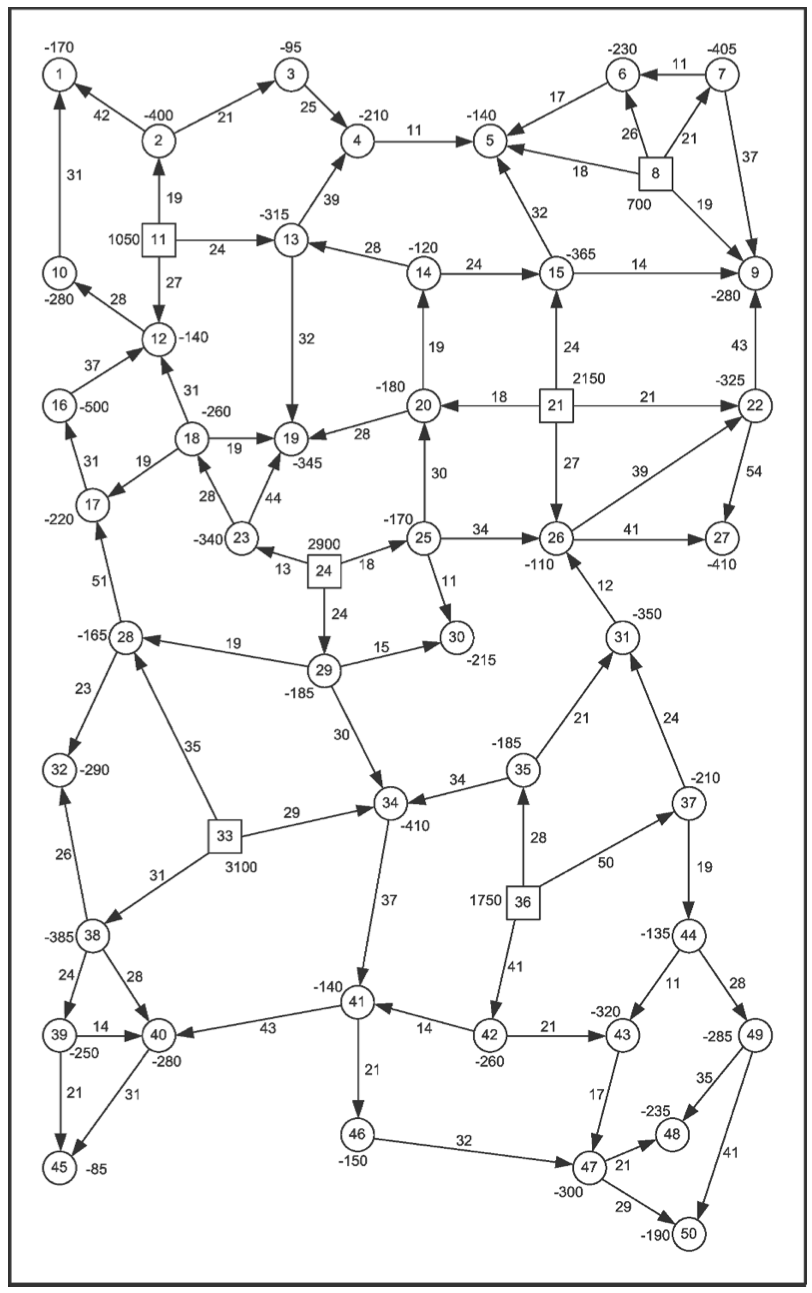
\includegraphics[scale=1]{./img/figure3-13.png}
	\caption{Supplies, demands (in units of 10 spools), and truck costs (in \texteuro) on a road map with 50 locations}
	\label{network3-1}
\end{figure}

\paragraph{(a)}
\begin{quote}
GTC wants to know a cheapest way of transporting spools to the cable depots in such a way that all depot demands are satisfied.
Since more spools are produced than are demanded, the company also wants to know which factories manufacture spools that are not shipped. How many spools are left at these factories?
\end{quote}

\paragraph{}
We find the minimum cost maximum flow in a network obtained from figure \ref{network3-1}. The capacities of arcs are infinite, the costs are taken from figure \ref{network3-1}. To 50 existing vertices we added a source and a sink. We added arcs from source to the 6 depots with zero costs and capacities equal to the number of spools in depots. We added arcs from all demand locations to sink with zero costs and capacities equal to the number of demanded spools. The number of spools left at factories can be found as the capacities of edges from source in residual network. We found minimum cost maximum flow and checked that it has saturated all arcs to the sink (i.e. all demand is satisfied).

\paragraph{}
For finding the minimum cost maximum flow we use Ford-Fulkerson-like algorithm that on each step finds the cheapest augmenting path using Ford-Bellman algorithm. We could have used Dijkstra's algorithm with potentials, but it would be an overkill for such small graph.

\paragraph{}
The flow (which is also a transportation plan) is shown in figure \ref{flow3-1a}. The minimum total cost is \texteuro 578535. The number of remaining spools is shown in table \ref{spools-left}.

\begin{figure}[H]
\centering
\begin{multicols}{5}
$ 2 \rightarrow 1 $ : 170

$ 2 \rightarrow 3 $ : 95

$ 8 \rightarrow 5 $ : 65

$ 8 \rightarrow 6 $ : 230

$ 8 \rightarrow 7 $ : 405
$ 11 \rightarrow 2 $ : 665
$ 11 \rightarrow 13 $ : 385
$ 12 \rightarrow 10 $ : 280
$ 13 \rightarrow 4 $ : 210
$ 14 \rightarrow 13 $ : 140
$ 15 \rightarrow 5 $ : 75
$ 15 \rightarrow 9 $ : 280
$ 17 \rightarrow 16 $ : 500
$ 18 \rightarrow 12 $ : 420
$ 18 \rightarrow 17 $ : 720
$ 20 \rightarrow 14 $ : 260
$ 20 \rightarrow 19 $ : 145
$ 21 \rightarrow 15 $ : 720
$ 21 \rightarrow 20 $ : 585
$ 21 \rightarrow 22 $ : 325
$ 21 \rightarrow 26 $ : 520
$ 23 \rightarrow 18 $ : 1400
$ 23 \rightarrow 19 $ : 200
$ 24 \rightarrow 23 $ : 1940
$ 24 \rightarrow 25 $ : 385
$ 24 \rightarrow 29 $ : 185
$ 25 \rightarrow 30 $ : 215
$ 26 \rightarrow 27 $ : 410
$ 33 \rightarrow 28 $ : 165
$ 33 \rightarrow 34 $ : 1420
$ 33 \rightarrow 38 $ : 1290
$ 34 \rightarrow 41 $ : 1010
$ 35 \rightarrow 31 $ : 350
$ 36 \rightarrow 35 $ : 535
$ 36 \rightarrow 37 $ : 630
$ 36 \rightarrow 42 $ : 585
$ 37 \rightarrow 44 $ : 420
$ 38 \rightarrow 32 $ : 290
$ 38 \rightarrow 39 $ : 335
$ 38 \rightarrow 40 $ : 280
$ 39 \rightarrow 45 $ : 85
$ 41 \rightarrow 46 $ : 870
$ 42 \rightarrow 43 $ : 325
$ 43 \rightarrow 47 $ : 5
$ 44 \rightarrow 49 $ : 285
$ 46 \rightarrow 47 $ : 720
$ 47 \rightarrow 48 $ : 235
$ 47 \rightarrow 50 $ : 190
\end{multicols}
\caption{Optimal transportation plan: the flow through each arc in tens of spools}
\label{flow3-1a}
\end{figure}

\begin{table}[H]
\centering
\begin{tabular}{|r|c|c|c|c|c|c|}
\hline
factory & 8 & 11 & 21 & 24 & 33 & 36 \\ \hline
spools & 0 & 0 & 0 & 390 & 225 & 0   \\ \hline
\end{tabular}
\caption{Number of spools left on each factory}
\label{spools-left}
\end{table}

\paragraph{(b)}
\begin{quote}
There are rumors that, because of the heavy traffic, the government is considering to levy toll on vehicles that use a certain road segment. It is not known yet which segment would be taxed, but road segments 38 $\rightarrow$ 40, 33 $\rightarrow$ 38, 12 $\rightarrow$ 10, 35 $\rightarrow$ 31, and 29 $\rightarrow$ 34 are considered as the most likely ones.
GTC is wondering whether the change of one road segment into a toll road will affect the cheapest transportation schedule from Problem 3.3(a). Determine for each of the above five road segments the maximum toll fee that can be charged on that segment without the current transportation plan becoming costlier than some other plan.
\end{quote}

\paragraph{}
We need to find the upper tolerance of some edges. To find the upper tolerance of an edge we set its capacity to the flow through it minus one and find the minimum cost maximum flow again. The difference between costs is the upper tolerance.

\paragraph{}
The maximum toll fees are given in table \ref{toll-fees}.

\begin{table}[H]
\centering
\begin{tabular}{|c|c|l|}
\hline
Arc & Fee & Comment \\ \hline
$ 38 \rightarrow 40 $ & 10 & \\ \hline
$ 33 \rightarrow 38 $ & 1 & \\ \hline
$ 12 \rightarrow 10 $ & $+\infty$ & can't reach 10 without this arc \\ \hline
$ 35 \rightarrow 31 $ & 25 & \\ \hline
$ 29 \rightarrow 34 $ & $+\infty$ & not in optimal plan \\ \hline
\end{tabular}
\caption{Maximum toll fees not changing the plan}
\label{toll-fees}
\end{table}

\paragraph{(c)}
\begin{quote}
There is also a possibility that the direction of traffic on the road segment 33~$\rightarrow$~34 will be reversed, i.e., it will become a one-way-traffic from 34 to 33. Determine a cheapest transportation plan under this new circumstance.
\end{quote}

\paragraph{}
The new plan is shown in figure \ref{flow3-1c}. Its cost is \texteuro 658175.

\begin{figure}[H]
\centering
\begin{multicols}{5}
$ 2 \rightarrow 1 $ : 170

$ 2 \rightarrow 3 $ : 95

$ 8 \rightarrow 5 $ : 65

$ 8 \rightarrow 6 $ : 230

$ 8 \rightarrow 7 $ : 405
$ 11 \rightarrow 2 $ : 665
$ 11 \rightarrow 13 $ : 385
$ 12 \rightarrow 10 $ : 280
$ 13 \rightarrow 4 $ : 210
$ 14 \rightarrow 13 $ : 140
$ 15 \rightarrow 5 $ : 75
$ 15 \rightarrow 9 $ : 280
$ 16 \rightarrow 12 $ : 310
$ 17 \rightarrow 16 $ : 810
$ 18 \rightarrow 12 $ : 110
$ 20 \rightarrow 14 $ : 260
$ 20 \rightarrow 19 $ : 145
$ 21 \rightarrow 15 $ : 720
$ 21 \rightarrow 20 $ : 585
$ 21 \rightarrow 22 $ : 325
$ 21 \rightarrow 26 $ : 520
$ 23 \rightarrow 18 $ : 370
$ 23 \rightarrow 19 $ : 200
$ 24 \rightarrow 23 $ : 910
$ 24 \rightarrow 25 $ : 385
$ 24 \rightarrow 29 $ : 1605
$ 25 \rightarrow 30 $ : 215
$ 26 \rightarrow 27 $ : 410
$ 28 \rightarrow 17 $ : 1030
$ 29 \rightarrow 34 $ : 1420
$ 33 \rightarrow 28 $ : 1195
$ 33 \rightarrow 38 $ : 1290
$ 34 \rightarrow 41 $ : 1010
$ 35 \rightarrow 31 $ : 350
$ 36 \rightarrow 35 $ : 535
$ 36 \rightarrow 37 $ : 630
$ 36 \rightarrow 42 $ : 585
$ 37 \rightarrow 44 $ : 420
$ 38 \rightarrow 32 $ : 290
$ 38 \rightarrow 39 $ : 335
$ 38 \rightarrow 40 $ : 280
$ 39 \rightarrow 45 $ : 85
$ 41 \rightarrow 46 $ : 870
$ 42 \rightarrow 43 $ : 325
$ 43 \rightarrow 47 $ : 5
$ 44 \rightarrow 49 $ : 285
$ 46 \rightarrow 47 $ : 720
$ 47 \rightarrow 48 $ : 235
$ 47 \rightarrow 50 $ : 190
\end{multicols}
\caption{Optimal transportation plan with reversed arc}
\label{flow3-1c}
\end{figure}
